%!TEX root = ../dissertation.tex

\chapter{Results}
\label{chp:results}
This chapter presents the results of employing the Social Media Kit (\textbf{SMKIT}) in real-world scenarios. The evaluation is structured to highlight both the strengths and the limitations of the system, providing a comprehensive view of its effectiveness in automating the process of generating and sharing social media content.


\section{Objectives Met}
\label{sec:objectives_met}
This section discusses the aspects of the \textbf{SMKIT} that successfully meet the objectives and goals. It highlights the features that have been successfully implemented and provide the intended functionality.

The following objectives have been successfully achieved by \textbf{SMKIT}:
\begin{itemize}
    \item \textbf{Metadata Extraction}: \textbf{SMKIT} successfully extracts metadata from web pages, including key Open Graph tags such as \texttt{og:title}, \texttt{og:description}, and \texttt{og:image}. This feature has been thoroughly tested across multiple websites, ensuring accurate extraction and processing of data required for social media posts.
    
    \item \textbf{Content Creation}: The system is capable of generating posts for various platforms, including Facebook, Twitter, and web pages. The posts are automatically formatted to meet platform-specific guidelines, ensuring consistency and correctness in terms of text length, image sizes, and other platform requirements.
    
    \item \textbf{Negapedia Integration}: \textbf{SMKIT} can generate posts specifically for Negapedia content. This includes generating summary posts, comparison posts, and ranking posts based on the data available in the Negapedia static pages. The system accurately processes Negapedia-specific data such as social interaction metrics and conflict-related data, ensuring high-quality posts for both social media platforms and web pages.
    
    \item \textbf{Social Media Integration}: The integration with the Facebook and Twitter APIs works seamlessly, enabling \textbf{SMKIT} to automatically post content to these platforms. The system correctly handles authentication and the posting process, ensuring that content is successfully shared with minimal manual intervention. The posts are also formatted to comply to each platform's specific content requirements.
\end{itemize}

In summary, \textbf{SMKIT} has successfully met the key objectives, demonstrating robust functionality in terms of metadata extraction, content generation for multiple platforms, and seamless integration with social media APIs.


\section{Improvement Areas}
\label{sec:improvement_areas}
This section identifies aspects of the \textbf{SMKIT} project that require improvement in order to create a more complete and efficient system. While \textbf{SMKIT} performs well in many areas, there are still challenges and limitations that need to be addressed. The following points highlight these areas for improvement:
\begin{itemize}
    \item \textbf{Platform Limitations}:
    Despite seamless integration with Facebook and Twitter, there were some limitations in specific platform functionalities, particularly with Twitter's occasional API post content check restrictions, which led to error response codes. Additionally, the system is currently only integrated with Facebook and Twitter, with no support for other popular platforms such as Instagram or LinkedIn. Expanding to these platforms could broaden the tool's reach and support a wider range of social media users.

    \item \textbf{Incomplete Metadata}:
    While \textbf{SMKIT} is successful in extracting the basic Open Graph metadata, such as title, description, and image, challenges remain in handling the full range of Open Graph tags. Currently, the system only extracts the basic tags required by the stakeholders. A potential improvement would be to expand the system's capabilities to handle all possible Open Graph tags, which would provide more comprehensive metadata for social media posts.

    \item \textbf{CLI Usability Improvement}: 
    The current command-line interface (CLI) is functional but not optimal for user experience. It requires technical knowledge to operate, making it challenging for less technically-inclined users. A significant improvement would be to develop a \textbf{Graphical User Interface (GUI)} to make the tool more user-friendly and accessible to a broader audience. This change would enhance the usability and overall experience of the system.

    \item \textbf{Social Post Metrics Calculation}: 
    Currently, \textbf{SMKIT} does not include functionality for calculating metrics related to social media posts, such as click-through rates, or engagement levels. Adding this functionality would provide valuable insights into the performance of posts, helping users evaluate the effectiveness of their content. This feature would significantly enhance the system's capabilities by allowing users to track and analyze the impact of their social media activity.
    
    \item \textbf{Error Handling Optimization}: There are opportunities to improve the system’s error handling. Currently, some error messages are not very informative, making it challenging to troubleshoot issues for less technically-inclined users. Enhancing the error handling system to provide more detailed and user-friendly error messages would improve the user experience.
\end{itemize}

In summary, while \textbf{SMKIT} performs well in many areas, there are still opportunities for improvement, particularly in platform integration, metadata extraction, and functionality expansion. Addressing these challenges—such as expanding platform support beyond Facebook and Twitter—will be essential for increasing the tool's reach and making it a more complete and efficient system in future versions.


\section{Social Media Post Examples and Web Pages}
\label{sec:social_media_post_examples_and_web_pages}
In this section, we present a few examples of posts generated by \textbf{SMKIT}. All combinations of modules and modes (such as Generic Module, Negapedia Module, and their respective Summary, Ranking, and Comparison modes) were created, but here we showcase only a few representative examples to illustrate the system's capabilities across different platforms.

\textbf{Generic Module - Summary Mode - Twitter Post}:  
This example shows a post created using the \textbf{Summary Mode} of the \textbf{Generic Module}, formatted for Twitter. The content is based on a selected web page, summarized to fit within Twitter’s accepted posts template.

\begin{figure}[H]
    \centering
    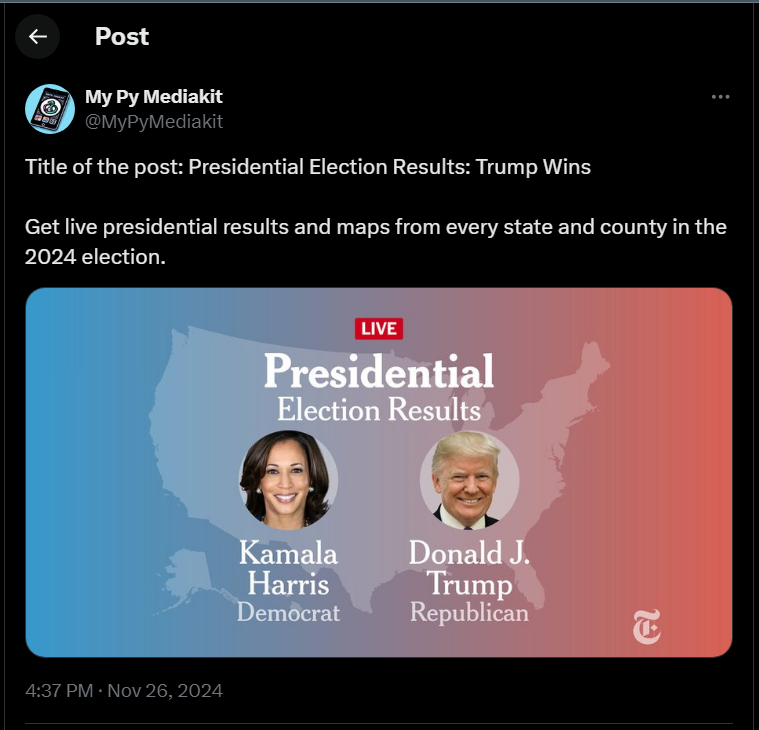
\includegraphics[width=0.8\textwidth]{figures/results/generic_module/summary_mode/twitter/twitter_generic_summary_post_screenshot.png}
    \caption{Twitter post generated by SMKIT using the Generic Module in Summary Mode.}
    \label{fig:twitter_generic_summary_post_screenshot}
\end{figure}

\textbf{Negapedia Module - Ranking Mode - Facebook Post}:  
This is an example of a post generated using the \textbf{Ranking Mode} of the \textbf{Negapedia Module}, formatted for Facebook. The post highlights the top-ranking topics on specific Negapedia data, designed to be visually engaging and informative for Facebook users.

\begin{figure}[H]
    \centering
    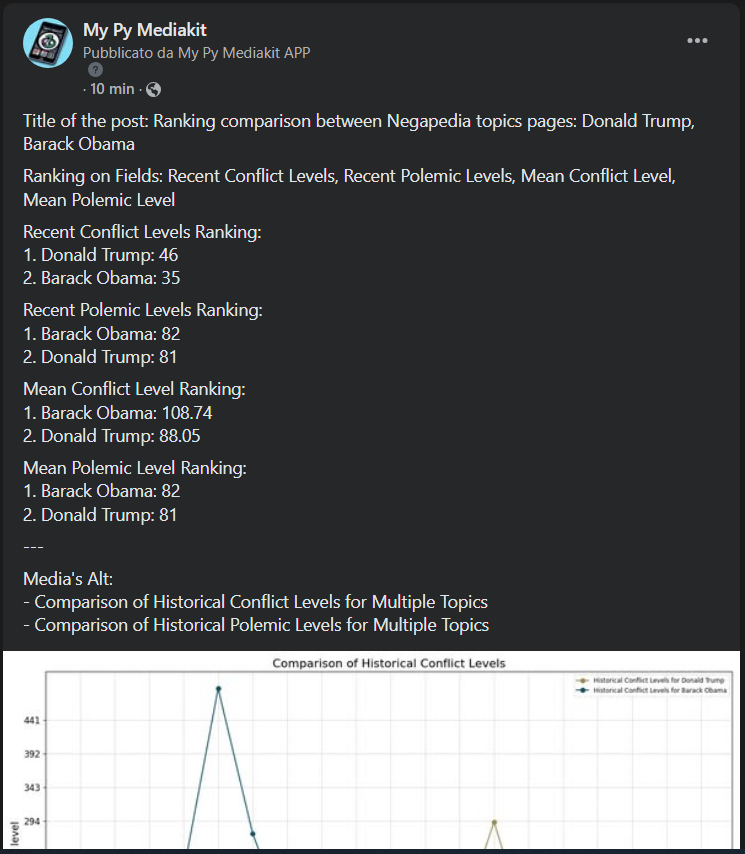
\includegraphics[width=0.8\textwidth]{figures/results/negapedia_module/ranking_mode/facebook/facebook_negapedia_ranking_post_screenshot.png}
    \caption{Facebook post generated by SMKIT using the Negapedia Module in Ranking Mode.}
    \label{fig:facebook_negapedia_ranking_post_screenshot}
\end{figure}

\textbf{Negapedia Module - Comparison Mode - Web Page Post}:  
This example shows a web page post generated using the \textbf{Comparison Mode} of the \textbf{Negapedia Module}. The post compares two Negapedia topics, highlighting key differences and similarities in metrics such as polemic and conflict scores. The web page version provides a detailed view of the comparison, with visual aids to support the analysis.

\begin{figure}[H]
    \centering
    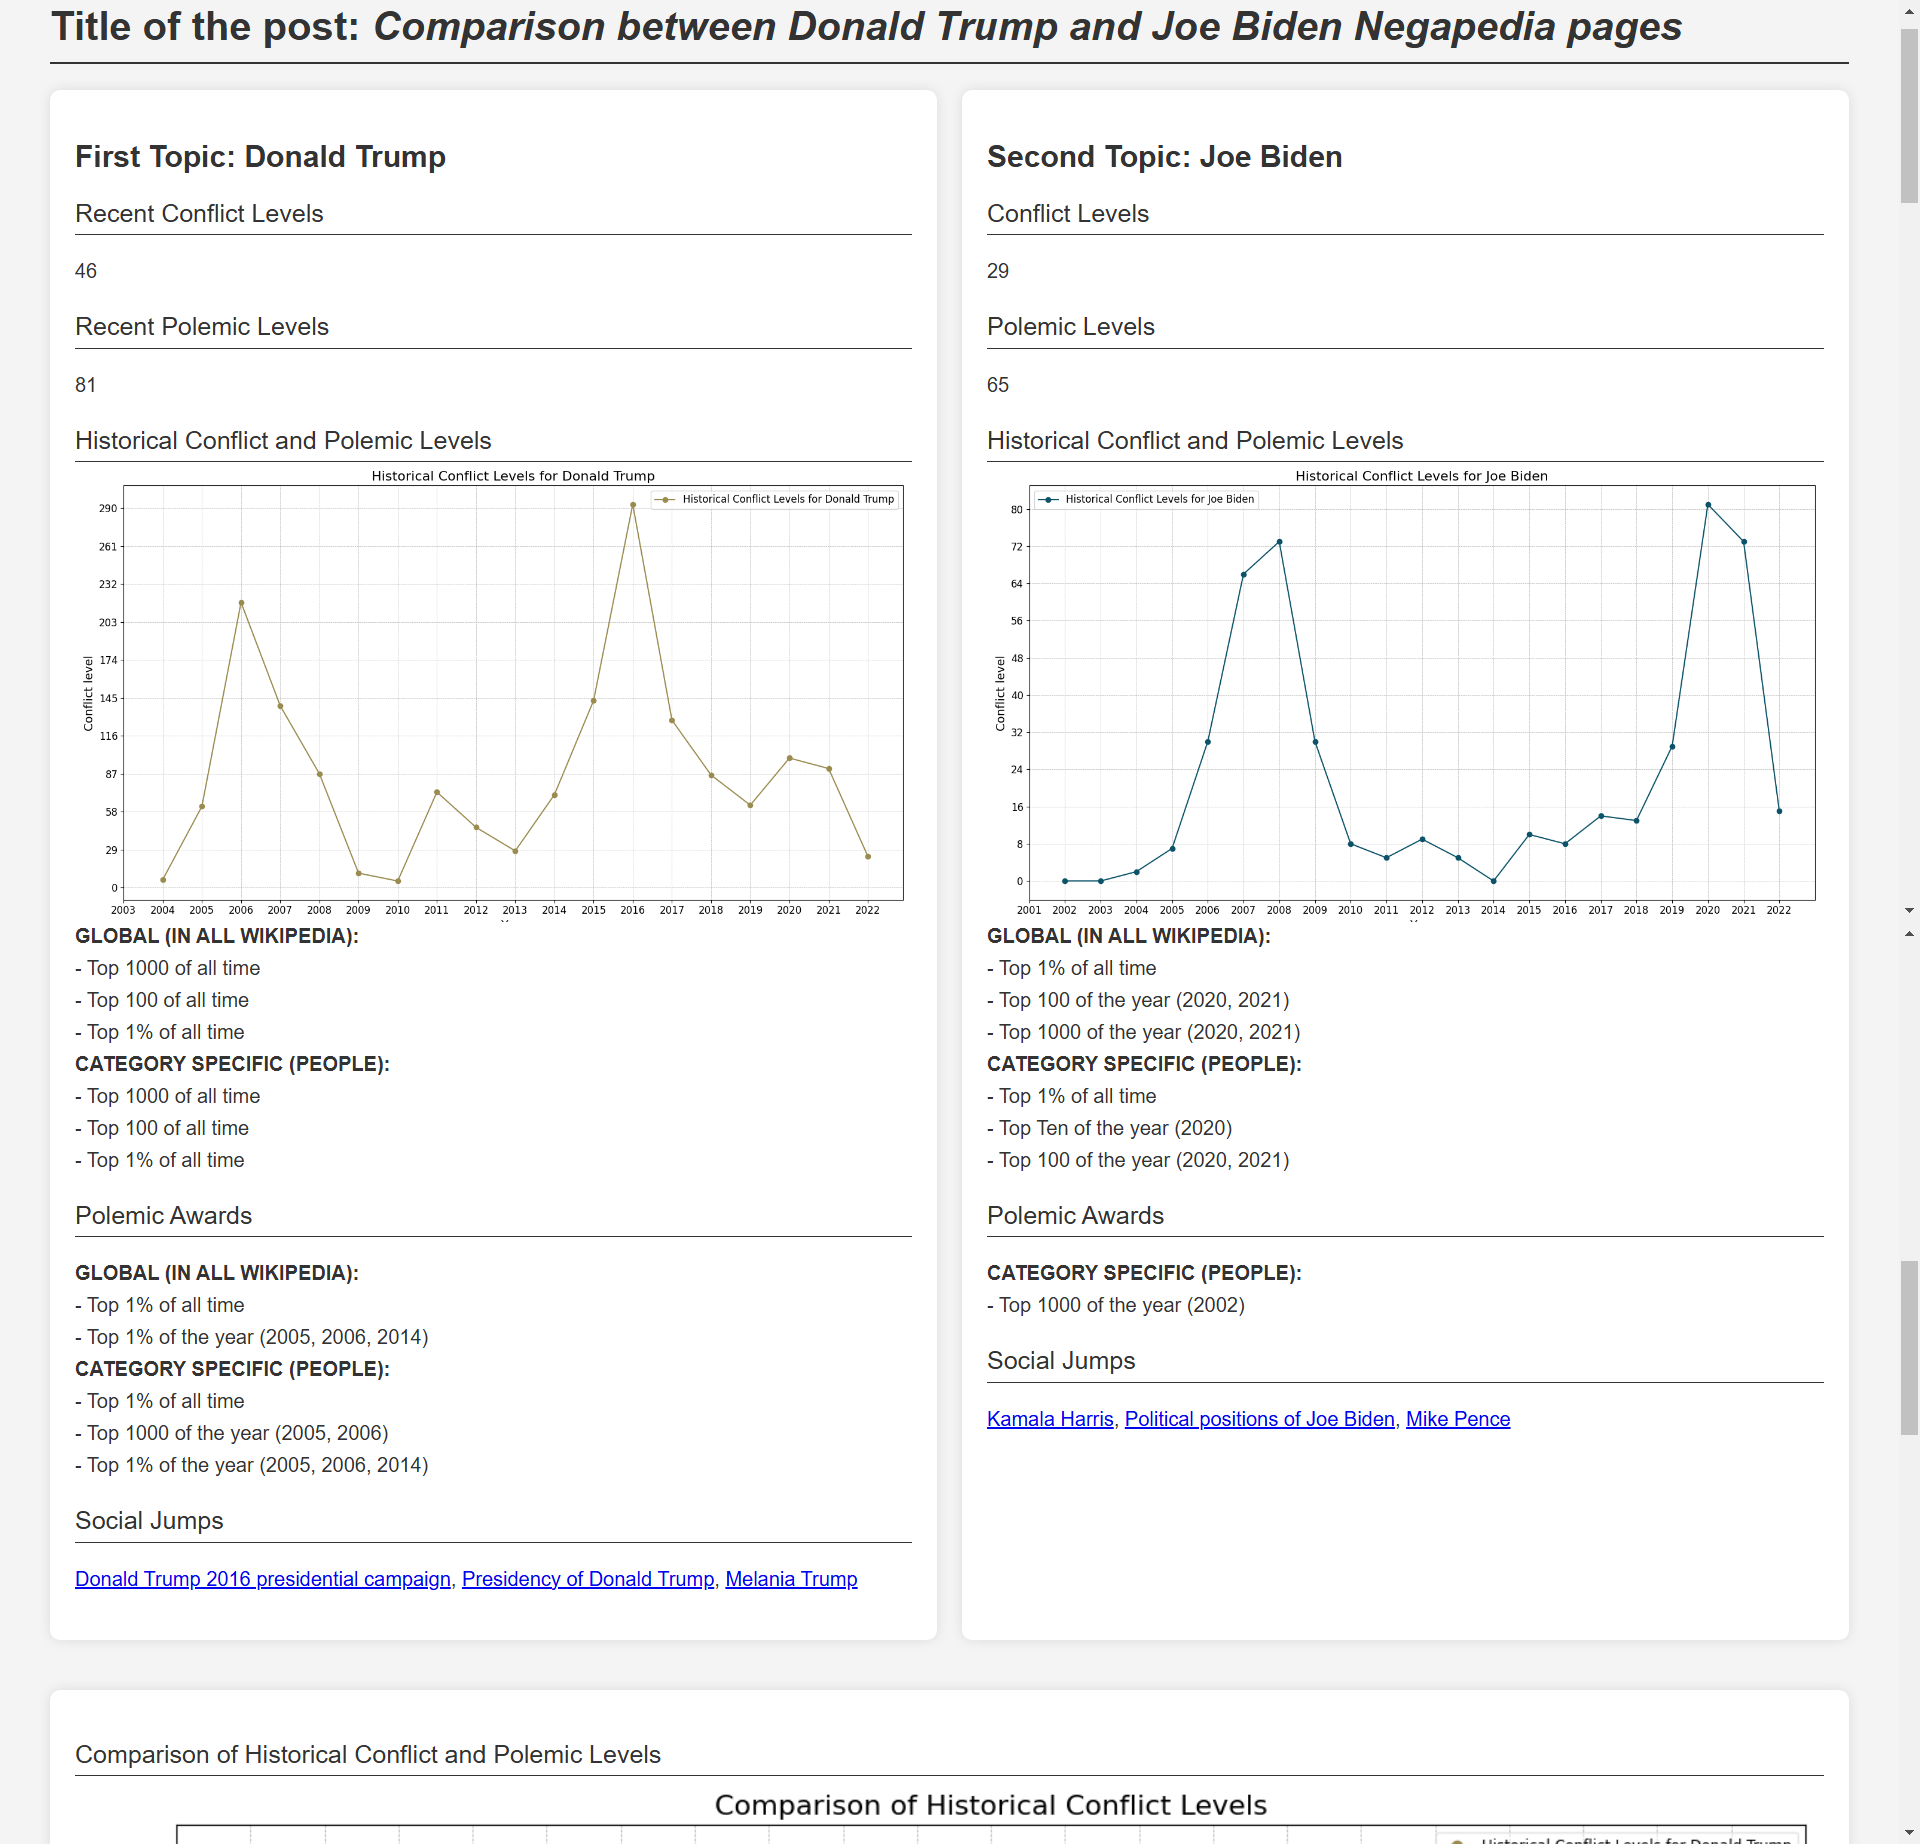
\includegraphics[width=0.8\textwidth]{figures/results/negapedia_module/comparison_mode/web_page/web_page_negapedia_comparison_post_screenshot.png}
    \caption{Web Page post generated by SMKIT using the Negapedia Module in Comparison Mode.}
    \label{fig:web_page_negapedia_comparison_post_screenshot}
\end{figure}

These examples demonstrate the system’s ability to create consistent and visually appealing posts across different platforms, highlighting the flexibility and potential of \textbf{SMKIT} in adapting content for various types of social media and web presentations.


\section{Execution Timing Analysis}
\label{sec:execution_timing_analysis}
This section presents an analysis of the execution time for different post types and operations within \textbf{SMKIT}. Below are the execution times for several post types, recorded during testing:

- \textbf{Generic Module - Summary Mode}: The execution time to generate and post content using the Generic Module in Summary Mode was \textbf{00:00:12.08} (12.08 seconds).

- \textbf{Negapedia Module - Summary Mode}: The execution time for creating a post using the Negapedia Module in Summary Mode was \textbf{00:00:14.82} (14.82 seconds), slightly longer than the Generic Module, as additional metadata processing for Negapedia content is involved.

- \textbf{Negapedia Module - Comparison Mode}: In Comparison Mode, where two topics are compared, the execution time was \textbf{00:00:31.47} (31.47 seconds). This is significantly longer than the other modes because the system processes more data and generates multiple visualizations (e.g., conflict and polemic visual scores), which requires more computational power.

- \textbf{Negapedia Module - Ranking Mode}: For Ranking Mode, which involves four topics, the execution time was \textbf{00:00:24.11} (24.11 seconds). This time is shorter than Comparison Mode, as the system retrieves the same data but processes it in different way.

Notably, the \textbf{Comparison Mode} should take longer than the \textbf{Ranking Mode}. This is due to the additional data processing and more complex plots required for comparison, whereas ranking works with the same data but performs lighter plots, which leads to faster execution times.


\section{Evaluation of Post Quality and Engagement}
\label{sec:evaluation_of_post_quality_and_engagement}
This section evaluates the quality and engagement of posts generated by \textbf{SMKIT}. 

\textbf{Post Quality}: The posts generated by \textbf{SMKIT} are designed to meet the specific formatting requirements of each platform, including Facebook, Twitter, and web pages. For Facebook and Twitter posts, \textbf{SMKIT} ensures that the character limits are adhered to, appropriate hashtags and mentions are included where relevant, and the posts are visually appealing. The web page posts are styled to maintain consistency with the content displayed on social media, while also being optimized for web presentation, ensuring proper layout and responsiveness. The system has been tested to handle varying lengths of text, media inclusion, and metadata presentation, producing consistent results across different platforms.

\textbf{Engagement Metrics}: Currently, we are unable to measure the engagement level of the generated posts. This limitation stems from the fact that \textbf{SMKIT} does not yet integrate with any systems that track social media engagement metrics such as likes, shares, or comments. Furthermore, the web pages generated by the system are not online and thus are not indexed by search engines or processed by SEO tools, limiting their visibility. Additionally, since the posts are not pushed through paid advertisement campaigns, they have not been exposed to a broad audience, which restricts any meaningful evaluation of engagement. Therefore, while the posts are designed to be engaging and platform-appropriate, we have not been able to gather any empirical data on their actual performance in terms of user interaction.


\section{Conclusion}
\label{sec:results_conclusion}
This section summarizes the key findings of the Results chapter. It provides a final assessment of how well \textbf{SMKIT} met the project objectives and performs in real-world usage. The conclusion also provides a transition to the next chapter, offering a perspective on **Future Work** or **Conclusions**.
